\chapter{Project Scope Management}

In this part, we will detail the project scope, clearly defining what is included and what is excluded from the project. We will also describe the development of the Work Breakdown Structure (WBS) and the Gantt chart for this project. These tools are essential for ensuring that the project remains focused on its intended goals and is executed efficiently without unnecessary expansion or deviation. By establishing these parameters, we aim to provide a structured approach to managing the project's scope, facilitating better control over project deliverables and timelines.


\section{Stakeholder Identification}
The first step before developing the project scope is to identify all stakeholders. This process ensures that the needs and expectations of every individual or group affected by the project are considered from the outset.

The stakeholders identified for the project are listed in Table \ref{tab:stakeholders}.


\begin{table}[h]
\centering
\caption{Stakeholders in the Recreation and Wellness Project}
\label{tab:stakeholders}
\begin{tabular}{|m{4cm}|m{8cm}|}
\hline
\textbf{Stakeholder} & \textbf{Role/Interest} \\
\hline
Employees & Direct beneficiaries, interested in wellness programs and facilities \\
\hline
Project Management Team & Responsible for planning, executing, and closing the project \\
\hline
Human Resources & Interested in employee satisfaction and retention \\
\hline
IT Department & Responsible for supporting technology needs and system integration \\
\hline
Health and Safety Officers & Ensure compliance with health and safety regulations \\
\hline
External Vendors & Provide necessary equipment or services for the wellness programs \\
\hline
Senior Management & Strategic oversight and funding decisions \\
\hline
\end{tabular}
\end{table}


\section{Requirements Analysis}

The next step in developing the project scope is to gather and list the requirements necessary for project completion. In this section, we will detail the requirement gathering process and present the requirements in a Requirement Traceability Matrix (RTM). This matrix will help ensure that each requirement is clearly linked to project objectives and can be traced throughout the project lifecycle.


\subsection{Requirements Gathering}

To ensure a thorough evaluation of all system aspects relevant to the project, requirements have been collected from various sources using diverse methods:

\begin{enumerate}
    \item \textbf{Stakeholder Interviews:} In-depth interviews with identified stakeholders are conducted to obtain detailed insights into their specific requirements and expectations.
    \item \textbf{Employee Surveys:} Surveys are distributed among employees to gather a broad spectrum of data on their perspectives and needs.
    \item \textbf{Focus Groups:} Focus group discussions are organized to explore particular issues or topics of interest in greater depth with a select group of stakeholders.
    \item \textbf{Review of Existing Systems and Data:} Current systems and historical data are analyzed to establish a baseline and identify potential areas for improvement.
    \item \textbf{Benchmarking:} Investigated and compared existing wellness programs or applications in other organizations to identify best practices and innovative features that could be incorporated into our project.

\end{enumerate}

\subsection{Requirement Traceability Matrix}

Once the requirements have been collected, we constructed a Requirement Traceability Matrix (RTM) to map each requirement back to its source. This matrix serves as a critical tool for ensuring that all requirements are clearly linked to their origins and that they are fully addressed throughout the project lifecycle. 

Table \ref{tab:rtm} list the Requirement Traceability Matrix (RTM) with its source and links it to specific features.

\begin{longtable}{|m{1cm}|m{5cm}|m{3.5cm}|m{3.5cm}|}
\caption{Requirement Traceability Matrix} \label{tab:rtm} \\
\hline
\textbf{ID} & \textbf{Requirement} & \textbf{Source} & \textbf{Feature} \\
\hline
\endfirsthead

\multicolumn{4}{c}%
{{\tablename\ \thetable{} -- \textit{Continued from previous page}}} \\
\hline
\textbf{ID} & \textbf{Requirement} & \textbf{Source} & \textbf{Feature} \\
\hline
\endhead
\endfoot

\hline
\endlastfoot

R1 & Develop a user-friendly interface for the wellness program application. & Stakeholder Interviews & User Interface Design \\
\hline
R2 & Ensure compliance with data privacy laws in health management applications. & Legal Requirements & Data Security \\
\hline
R3 & Implement a system for tracking employee participation in wellness activities. & Employee Surveys & Activity Tracking \\
\hline
R4 & Integrate third-party services for mental health resources. & Focus Groups & Third-Party Integration \\
\hline
R5 & Create a feedback mechanism for users to report issues and suggestions. & Employee Surveys & User Feedback System \\
\hline
R6 & Enable customization of wellness programs to meet individual health goals. & Stakeholder Interviews & Personalization Settings \\
\end{longtable}

\section{Project Scope Statement - Version 1}

This section presents the initial version of the project scope statement as created by the project manager. The document outlines key project objectives, deliverables, and the overall approach.

\includepdf[pages=-]{parts/part2/scope.pdf}

\section{Work Breakdown Structure}

A comprehensive Work Breakdown Structure (WBS) has been developed to systematically organize and define the total scope of the "Recreation and Wellness Intranet" project. This structure delineates all key deliverables and breaks them down into manageable components, facilitating more effective planning and execution.

The WBS for our project is meticulously organized into five distinct phases, each tailored to ensure structured progress and effective management throughout the project lifecycle. These phases are as follows:

\begin{enumerate}
    \item \textbf{Initiation:}
        \begin{itemize}
            \item Proposal: Document the initial proposal provided by MYH.
            \item Project Analysis: Perform initial feasibility and scope analysis.
            \item Objectives Analysis: Align project objectives with strategic goals.
            \item Proposal Reanalysis: Refine the proposal based on initial findings.
            \item Financial Analysis: Calculate financial metrics like NPV and ROI.
            \item Business Case: Develop and finalize the business case.
        \end{itemize}

    \item \textbf{Planning:}
        \begin{itemize}
            \item Stakeholder Identification: Identify and document all key stakeholders.
            \item Requirements Analysis: Detailed analysis of project requirements.
            \item Requirement Gathering: Collection of specific system requirements.
            \item Requirement Traceability Matrix: Creation of an RTM.
            \item Project Scope: Development of a detailed project scope document.
            \item Work Breakdown Structure: Create a detailed WBS for task organization.
            \item Gantt Chart: Develop a Gantt chart to outline project timelines.
        \end{itemize}

    \item \textbf{Execution:}
        \begin{itemize}
            \item Project Quality Documentation: Set standards for project quality.
            \item Project Resource Documentation: Document all project resources.
            \item Project Risk Documentation: Assess and document project risks.
            \item UML Diagram and System Design: Create UML diagrams and system designs.
        \end{itemize}

    \item \textbf{Monitoring and Control:}
        \begin{itemize}
            \item Standard Draft Preparation: Develop standardized document templates.
            \item Version Control: Implement version control systems like GitHub.
            \item Performance Tracking: Monitor project performance against planned metrics.
        \end{itemize}

    \item \textbf{Closure:}
        \begin{itemize}
            \item Final Documentation: Compile comprehensive project documentation.
            \item Presentation: Prepare and deliver the final project presentation to MYH leadership.
        \end{itemize}

    \item \textbf{Post-Project Evaluation:}
        \begin{itemize}
            \item Evaluate project outcomes against initial objectives.
            \item Document lessons learned and provide recommendations for future projects.
        \end{itemize}
\end{enumerate}

Each of these phases plays a crucial role in the structured and successful delivery of the project, ensuring that all objectives are met and the project delivers the intended benefits.

Figure \ref{fig:wbs} provides a visual representation of the Work Breakdown Structure in the form of a flowchart, illustrating the hierarchical organization of project tasks.

\begin{figure}[ht]
    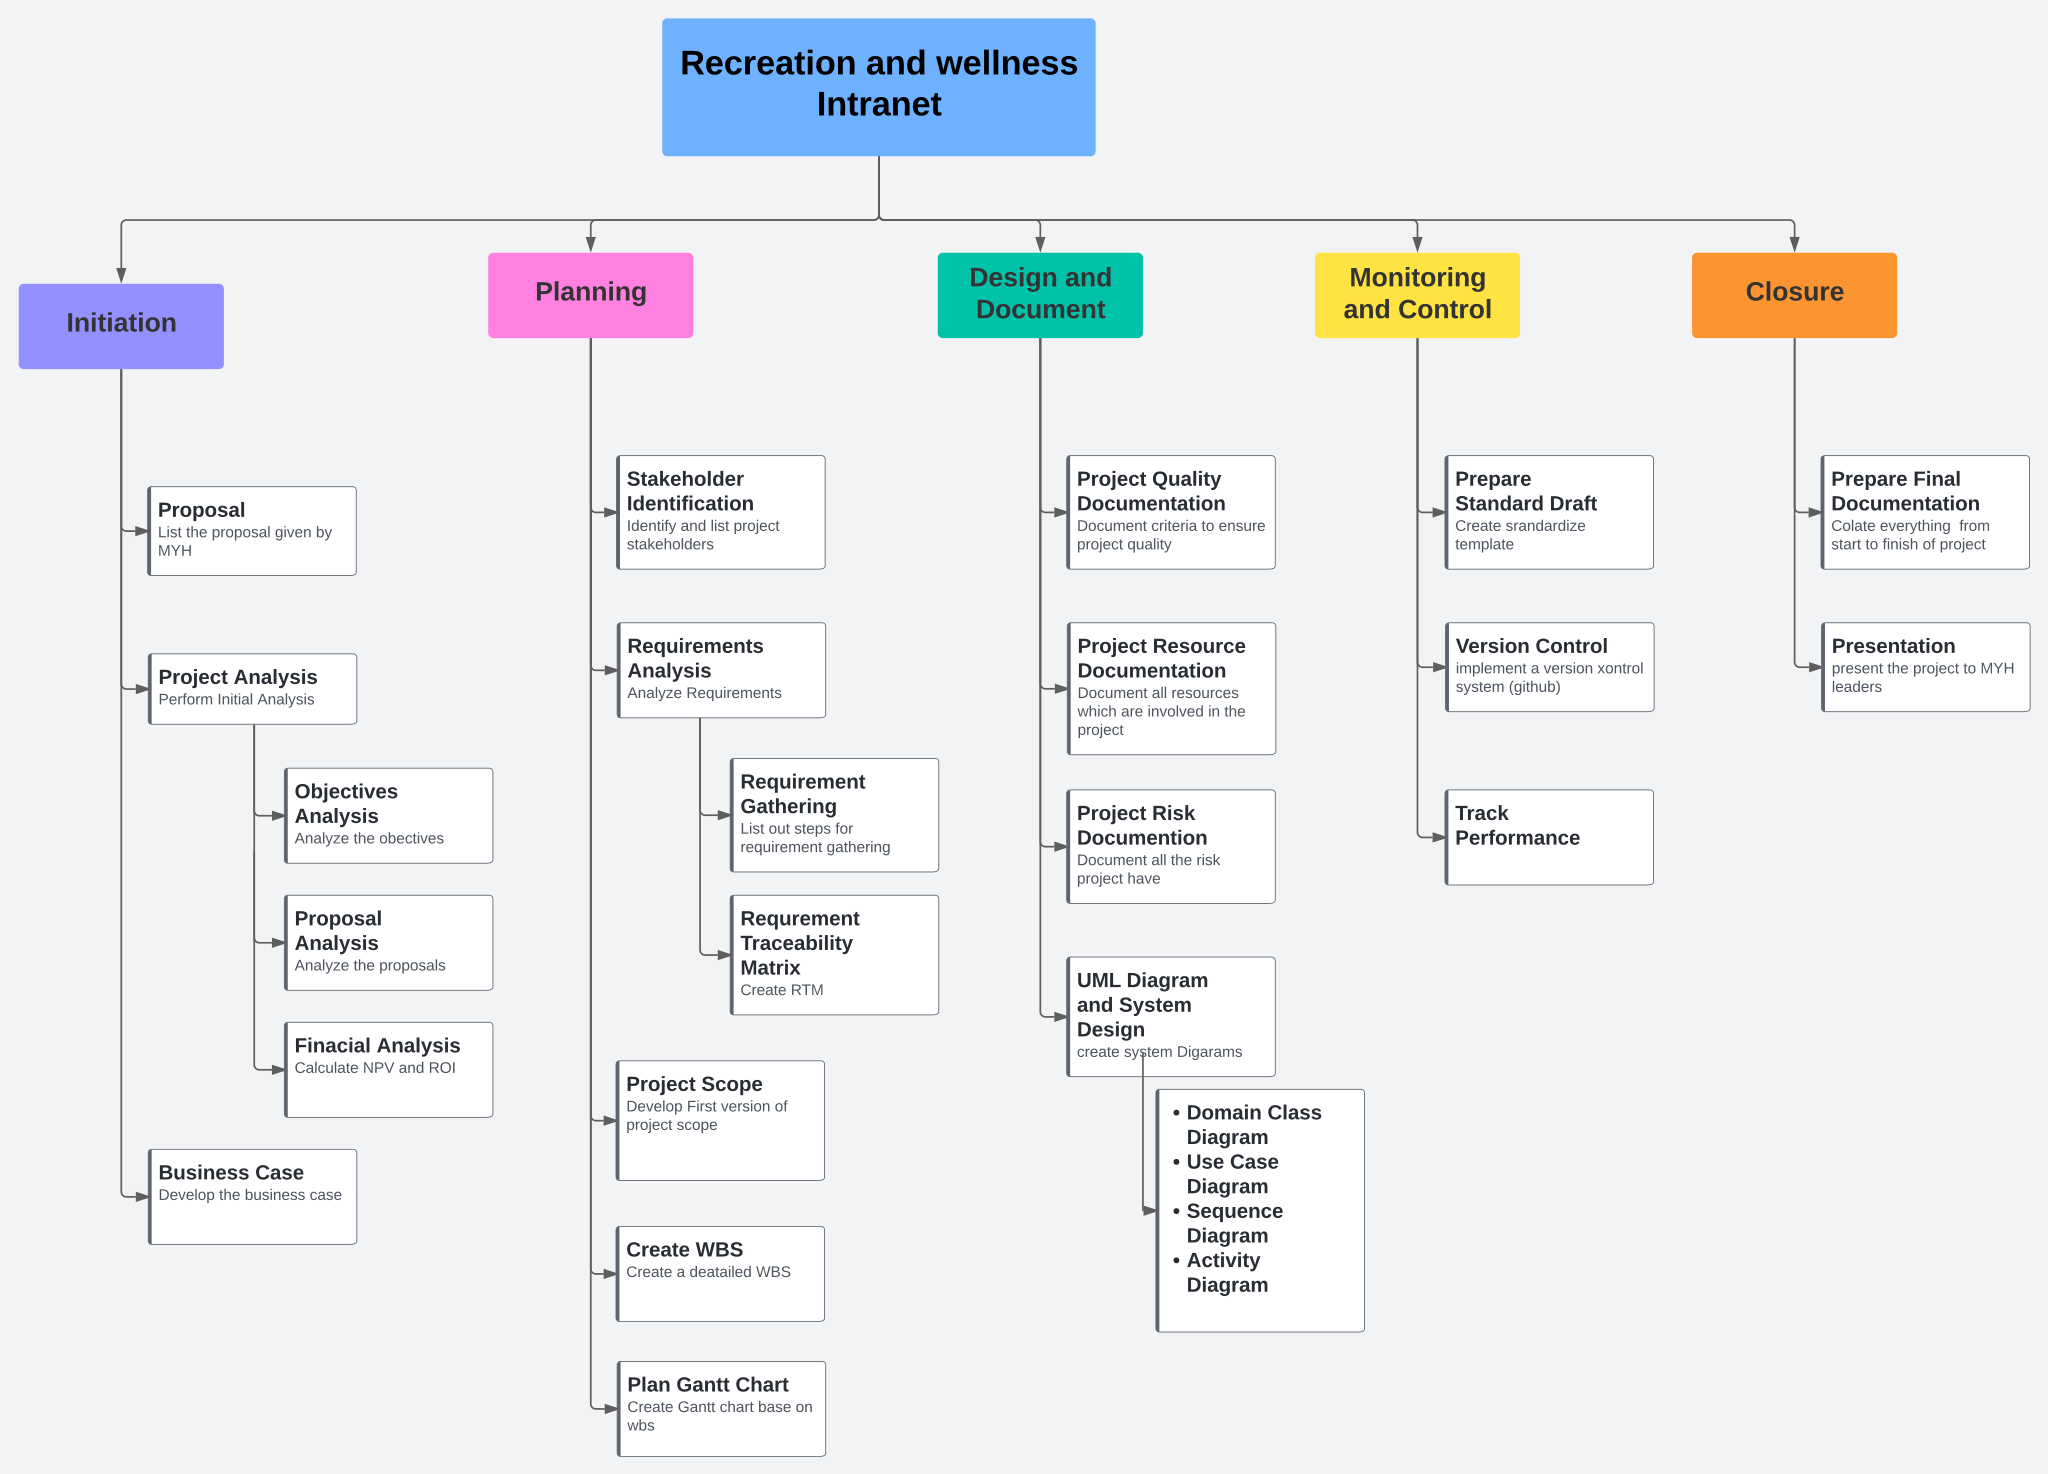
\includegraphics[width=\textwidth]{images/wbs.png}
    \caption{Work Breakdown Structure}
    \label{fig:wbs}
\end{figure}

\section{Initial Gantt Chart}

The initial Gantt chart, which outlines the project task and dependencies, is depicted in Figure \ref{fig:gnt1} and \ref{fig:gnt2}.

\begin{figure}[ht]
    \includegraphics[width=\textwidth]{images/gantt_2.png}
    \caption{Gantt Chart}
    \label{fig:gnt1}
\end{figure}

\begin{figure}[ht]
    \includegraphics[width=\textwidth]{images/gantt_1.png}
    \caption{Gantt Chart}
    \label{fig:gnt2}
\end{figure}

\FloatBarrier
\newpage